\section{Calorimeter Window Size}\label{app:window_size}

The optimal window size to store for ECAL and HCAL is an important issue, since this impacts not only sample storage size, but also training speed and the maximum batch sizes which we could feed to our GPUs. 

From examinations of our generated samples, we found that an ECAL window of 25x25x51 and an HCAL window of 11x11x60 looked reasonable. To test this hypothesis, we performed training using the samples and classification architectures described in our previous studies~\cite{NIPS}, but with different-sized input samples. The architecture was altered to accommodate larger windows simply by increasing the number of neurons on the input layer. Results trained using an ECAL window of size 25x25x25 and 51x51x25 are shown in Figure~\ref{fig:classification_window}. From the similarity of these curves, we have decided that an expanded ECAL window size does not contain much additional useful information, and is thus not necessary for our problems.

\begin{figure*}[htbp]
\centering
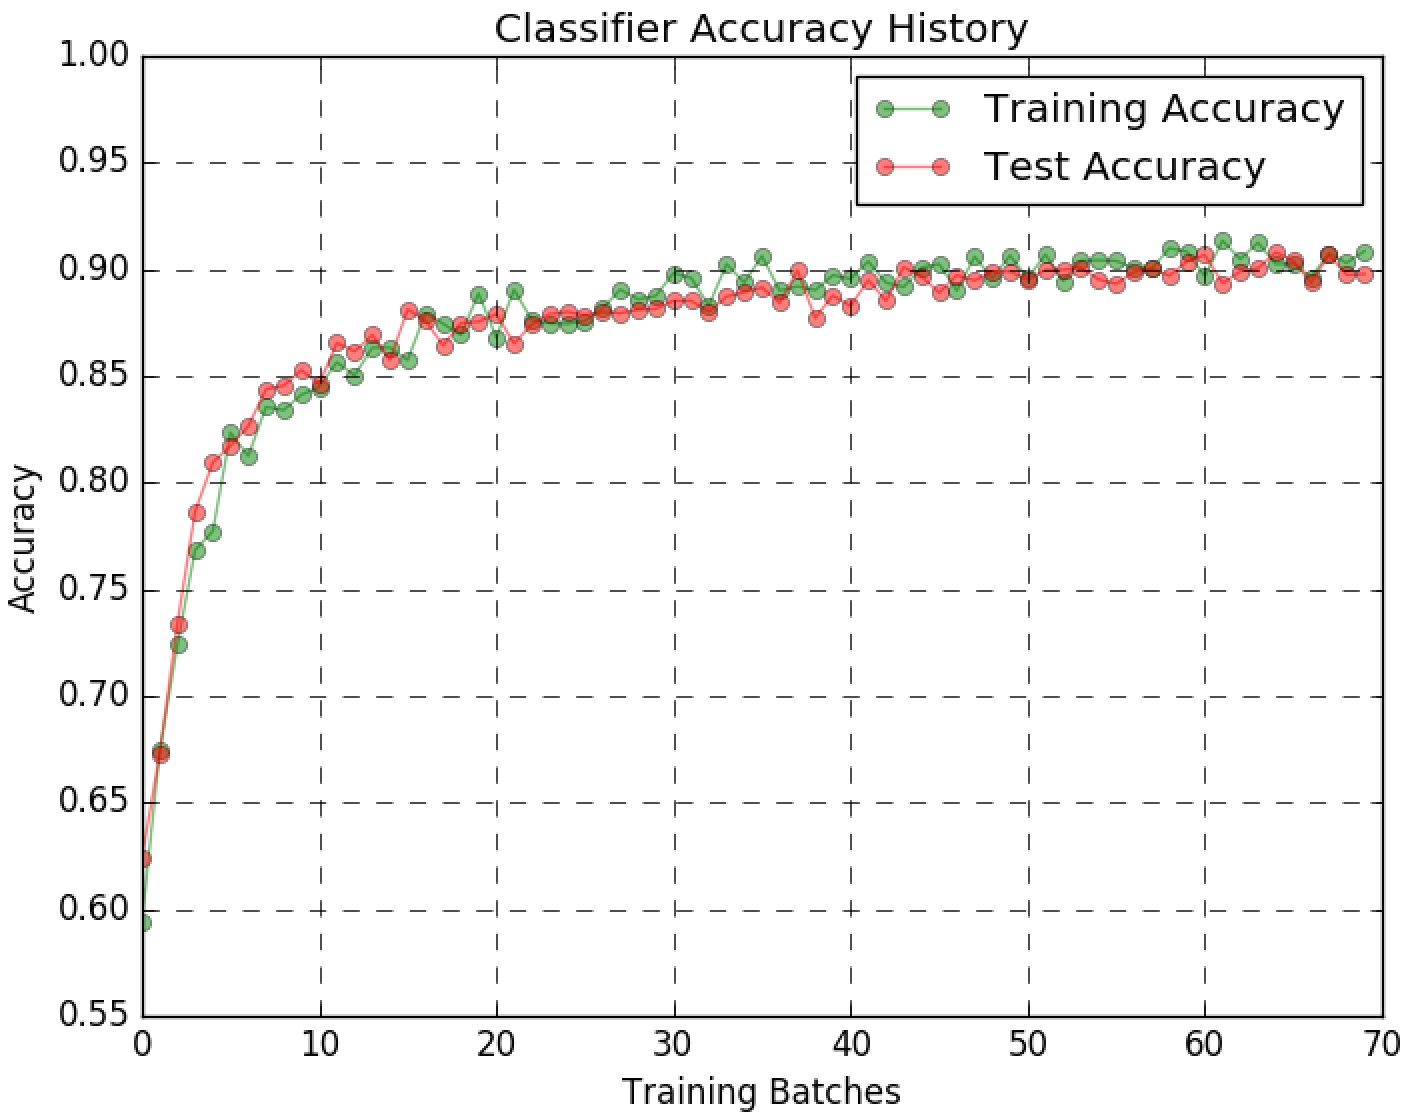
\includegraphics[width=0.38\textwidth]{images/accuracy_small_window.png}
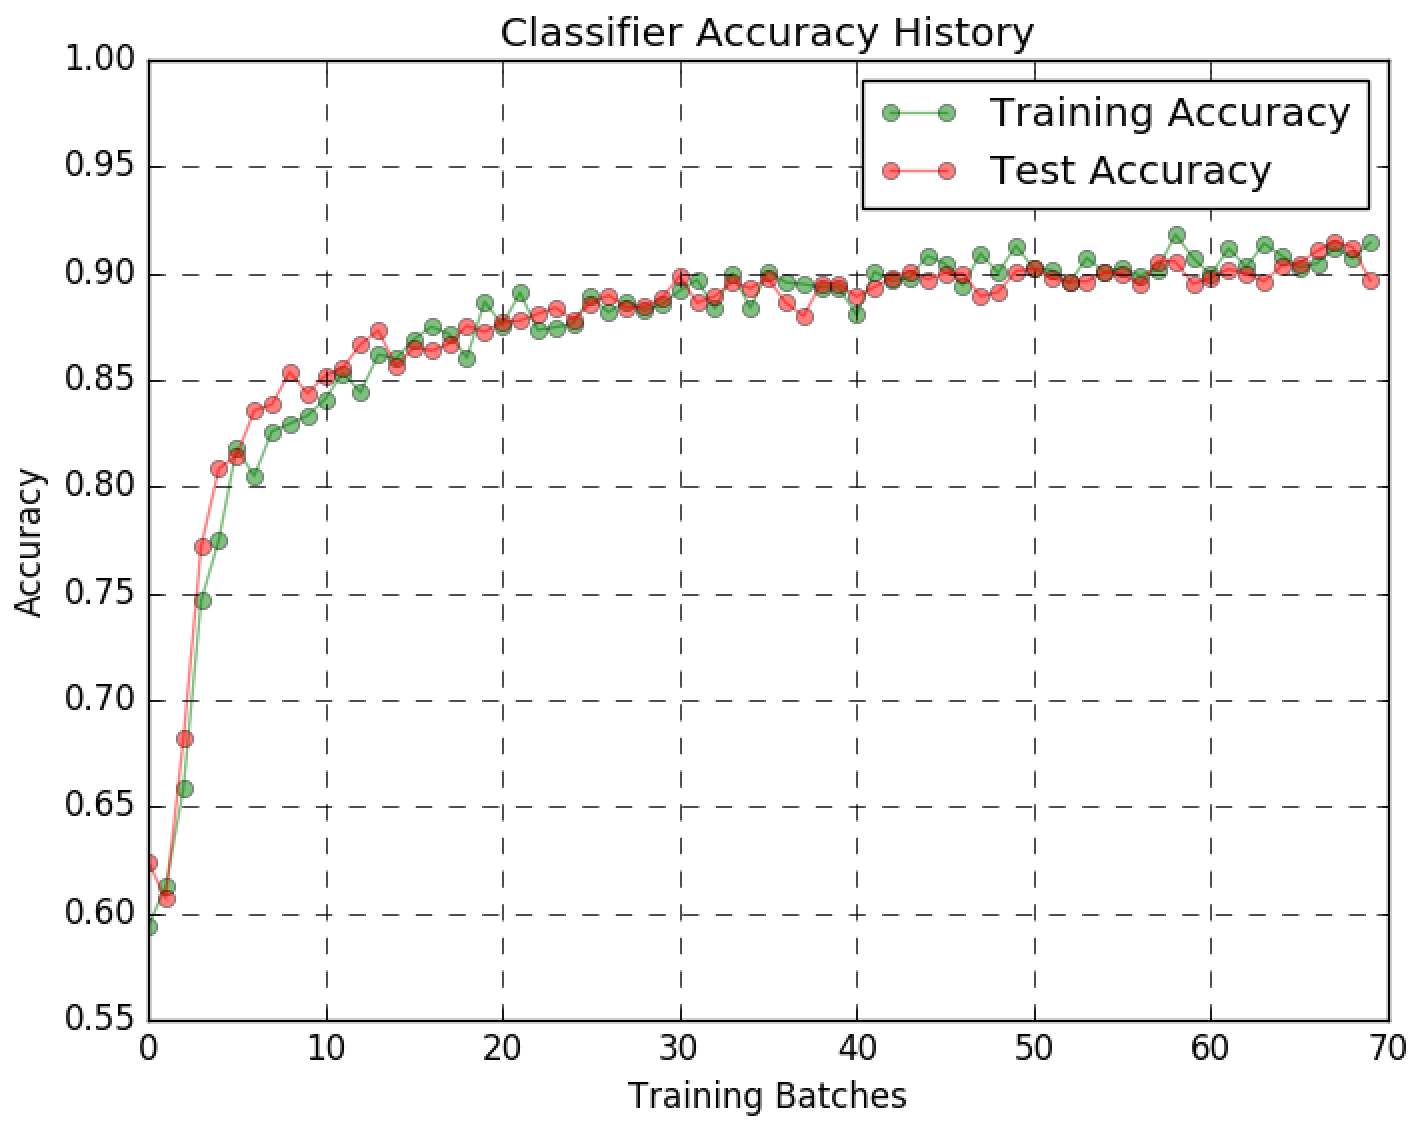
\includegraphics[width=0.38\textwidth]{images/accuracy_large_window.png}
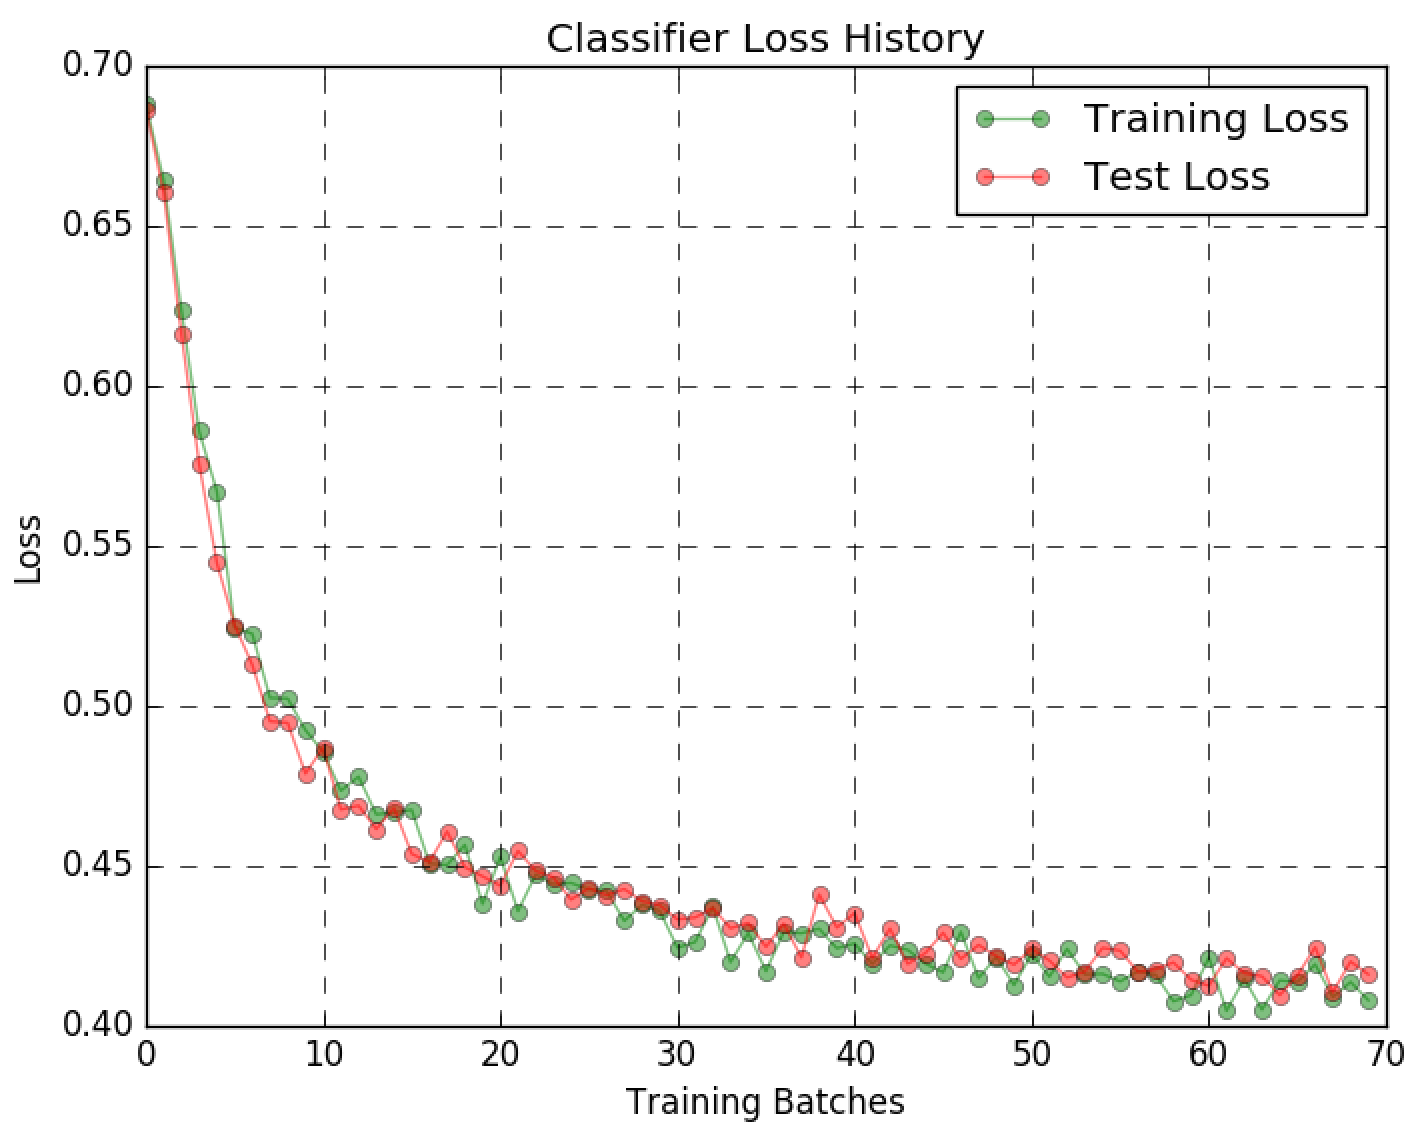
\includegraphics[width=0.38\textwidth]{images/loss_small_window.png}
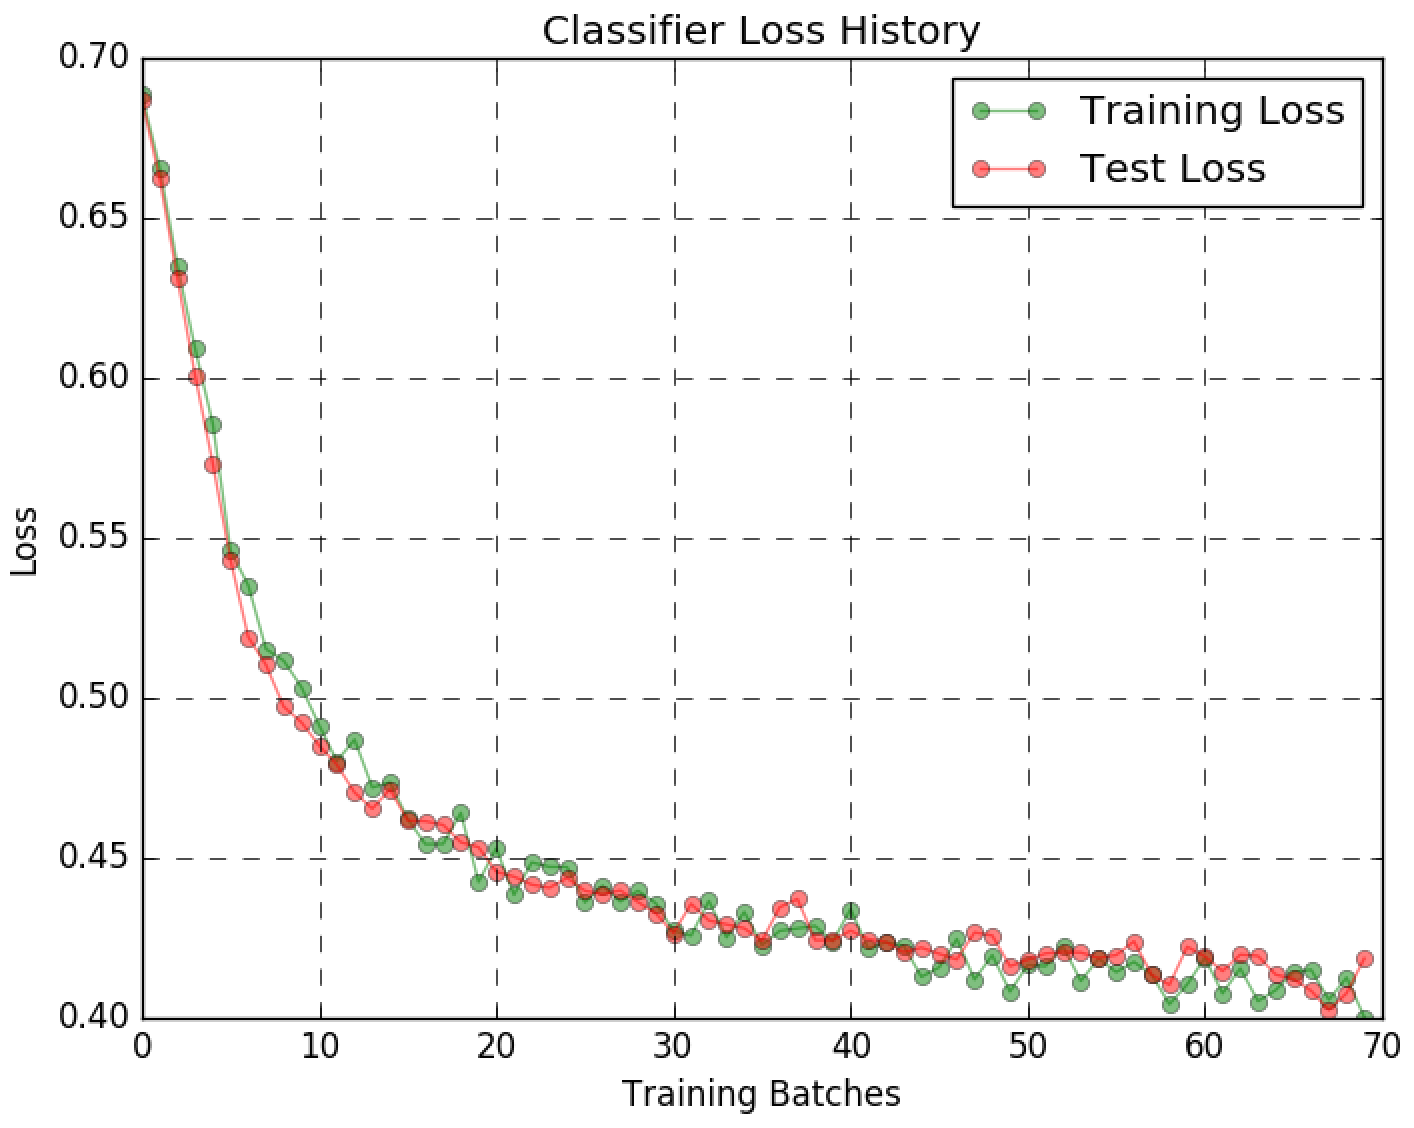
\includegraphics[width=0.38\textwidth]{images/loss_large_window.png}
\caption{Training history for different choices of the input 3D array zise: Accuracy (top) and loss (bottom) as a function of the training batch for photon/neutral pion classification, using a 25x25x25 (left) and 51x51x25 (right) ECAL window size.\label{fig:classification_window}}
\end{figure*}